%\date{\copyright\today}
\documentclass[fontsize=12pt,a4paper]{scrartcl}[2003/01/01]

% Das Prozent-Zeichen leitet einen Kommentar ein,
% es hilft ebenso, im Text Leerzeichen zu unterbinden.

% fontsize=12pt  Schriftgroesse in 10, 11 oder 12 Punkt
% a4paper        Papierformat ist hier A4
% landscape      Querformat wird natürlich unterstützt ;-)
% parskip        Absatzabstand anstatt Einzüge
% draft          Der Entwurfsmodus deckt Schwächen auf
% {scrartcl}     Die Dokumentenklasse book, report, article
%                oder fürs deutsche scrbook, scrreprt, scrartcl

\usepackage[ngerman]{babel} % Deutsche Sprachanpassungen
\usepackage[T1]{fontenc}    % Silbentrennung bei Sonderzeichen
\usepackage[utf8]{inputenc} % Direkte Angabe von Umlauten im Dokument.
                            % Wenn Sie an einem Mac sitzen,verwenden
                            % Sie ggf. „macce“ anstatt „utf8“.

\usepackage{textcomp}       % Zusätzliche Symbolzeichen
\usepackage{blindtext}      % Blindtext zum Testen von Textausgaben
\usepackage{float}
\usepackage{graphicx}
\usepackage{tabularx}
\usepackage[german]{datetime2}

% Git Info
%\usepackage[local,missing={(Oh my!)},dirty={Oh no!},markifdirty,marknotags]{gitinfo2}
\usepackage[missing={(Oh my!)},dirty={Oh no!},mark]{gitinfo2}

\title{LastShelter: Survival}
\subtitle{Farming Guide}
\author{\textcopyleft{} anmiwa (Reich449)%
  \thanks{Mit den besten Empfehlungen, PAt Pain Attac}}
\date{\DTMfetchday{gitdate}. \DTMgermanmonthname{\DTMfetchmonth{gitdate}} \DTMfetchyear{gitdate}}

\usepackage[%
	bookmarksnumbered,
	bookmarksopen,
	linktocpage,
	]{hyperref}
\hypersetup{
   pdfauthor={(PAt) anmiwa [State 449]},
   pdftitle={LastShelter: Survival: Farming Guide},
   pdfsubject={Eine Anleitung um viele Farmen in LastShelter zu betreiben.},
   pdfkeywords={lastshelter;farm},
}

\begin{document}
\maketitle                  % Titelei erzeugen

%{\centering
%Release:\gitReln\ (\gitAbbrevHash)\\
%}
% -----------------------------------------------------
\thispagestyle{empty}
\pagebreak
\tableofcontents*            % Inhaltsverzeichnis anlegen
\listoffigures
\pagebreak
% -----------------------------------------------------

\section{Einleitung}
Hier will ich euch eine Anleitung an die Hand geben, wie ihr Farmen für eure Main-Basis anlegen könnt.
Ab dem Level 16 wird es sehr schwer die notwendigen Ressourcen durch Plündern von Gegnern zu bekommen.
Ein starker Gegner kann einem auch am Ende mehr kosten als nutzen. Dasselbe gilt für Zombies.

Sammeln an den Ressourcen-Stationen ist sehr langwierig und bindet die APC für das Sammeln.
Kurz um ihr braucht früher oder später Farmen um voran zu kommen.

Top Spieler mit Level 20 und höher haben zum Teil mehr als 30 Farmen! Ich denke aber für den Anfang sind 3 bis 4 ausreichend.

Da man viel Zeit bräuchte wenn man jede Farm täglich bewirtschaften müsste, ist das Ziel Farmen zu bauen,
die maximal einmal pro Woche kurz bearbeitet werden. Das könnte Donnerstag oder Sonntag sein,
da hier der Helden Event läuft, der viele Ressourcen für die Farm bringen kann.
Siehe Helden-Event~\ref{Heldenevent} auf der Seite~\pageref{Heldenevent}.

\begin{table}[ht]
  \centering
    \begin{tabularx}{0.6\textwidth}{rl}
      Ressource & Tagesproduktion \\
      \hline
      Nahrung & 2.267 k \\
      Wasser & 2.340 k \\
      Öl & 1.883 k \\
      Strom & 213 k \\
      Holz & 1.490 k \\
      Eisen & 952 k \\
      Geld & 912 k \\
    \end{tabularx}
  \caption[Ertrag]{Täglicher Ertrag einer fertigen Farm}
\end{table}


\section{Die Farm}
\subsection{Farm anlegen}
Eine Farm wird angelegt indem man ein neues Spiel startet. Dies kannst du unter Einstellungen/Konto machen.
Jetzt musst du die Einführung ganz normal durchspielen. Bis einschließlich Level 5 hast du einen Schutzschirm,
also gehe nicht auf Level 6 (Abbildung~\ref{fig:aufgaben}) bevor du nicht in unserer Allianz bist und wir dich in unseren Hive transportiert haben.

\begin{figure}[H] 
  \centering
     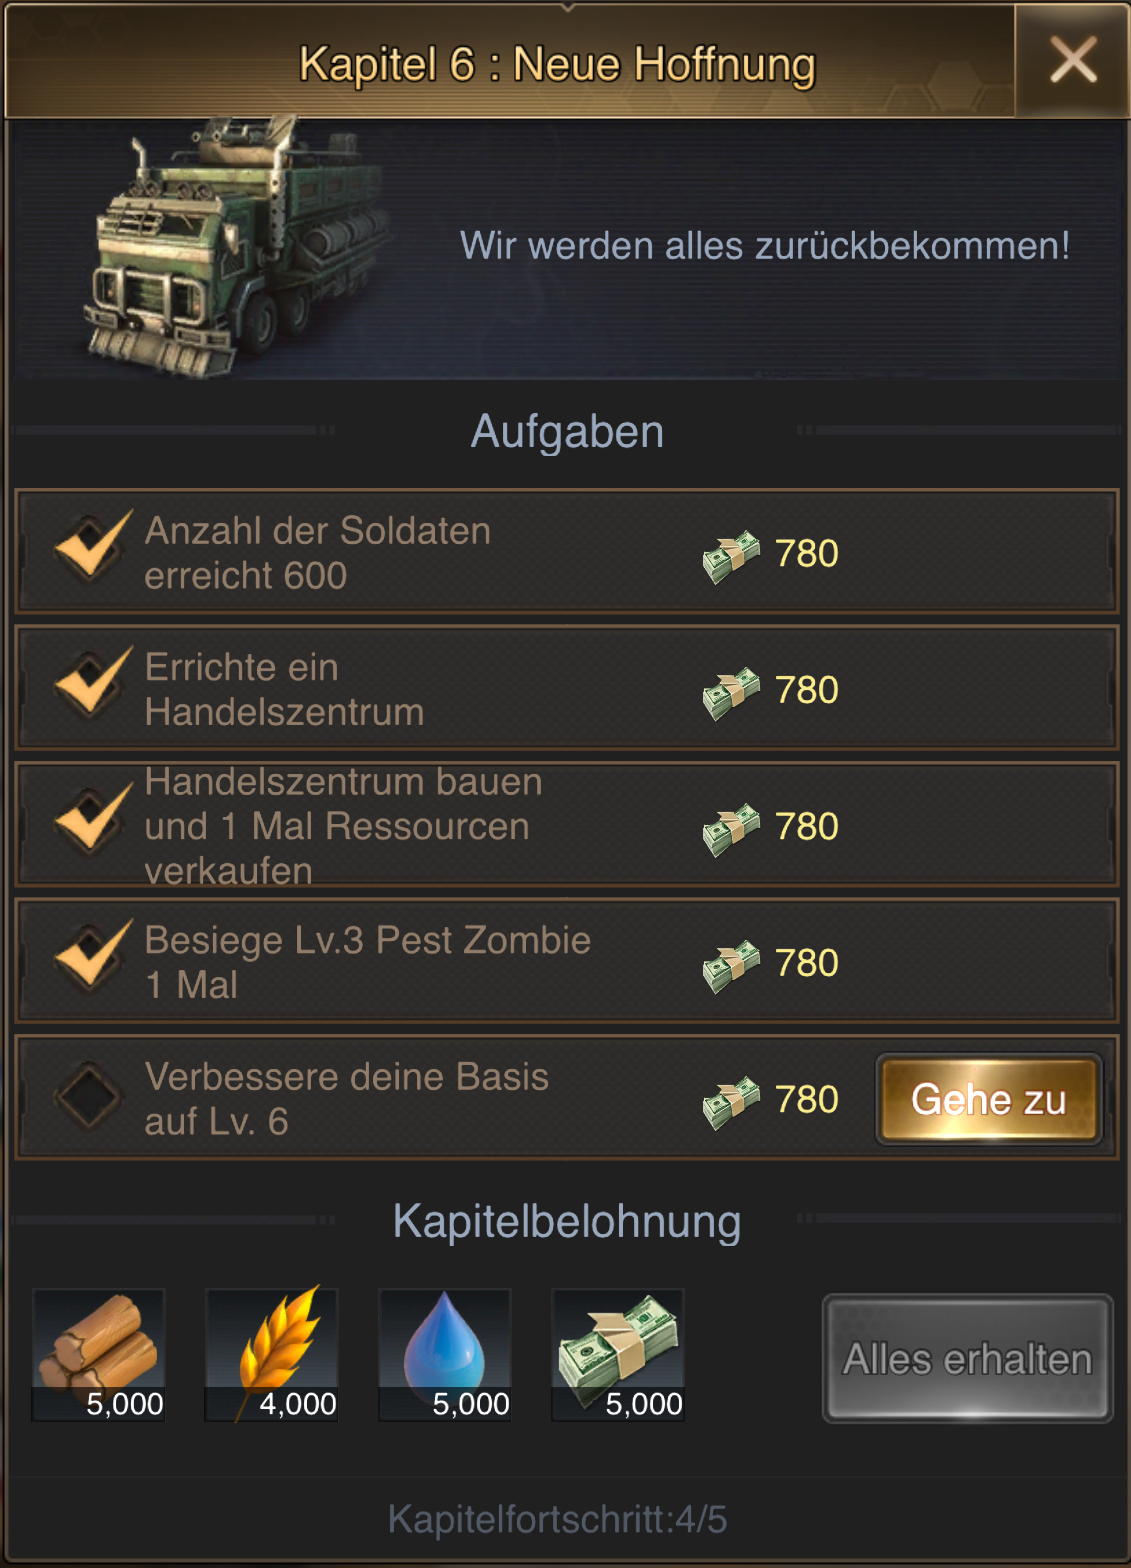
\includegraphics[width=5cm]{Bilder/IMG_E0002.JPG}
  \caption{Aufgaben}
  \label{fig:aufgaben}
\end{figure}

Deine Farm ist in einem zufälligen Reich (Staat). Du musst also in unseren umziehen. Dazu gehst du auf die Weltkarte.
Unten in der Mitte findest du ein Feld mit den aktuellen Koordinaten. Da klickst du drauf. Jetzt öffnet sich ein 
Fenster (Koordinaten eingeben) in dem du das Reich 449 eintragen musst. X und Y sind erst mal egal. (Abbildung~\ref{fig:koordinaten})

\begin{figure}[H] 
  \centering
     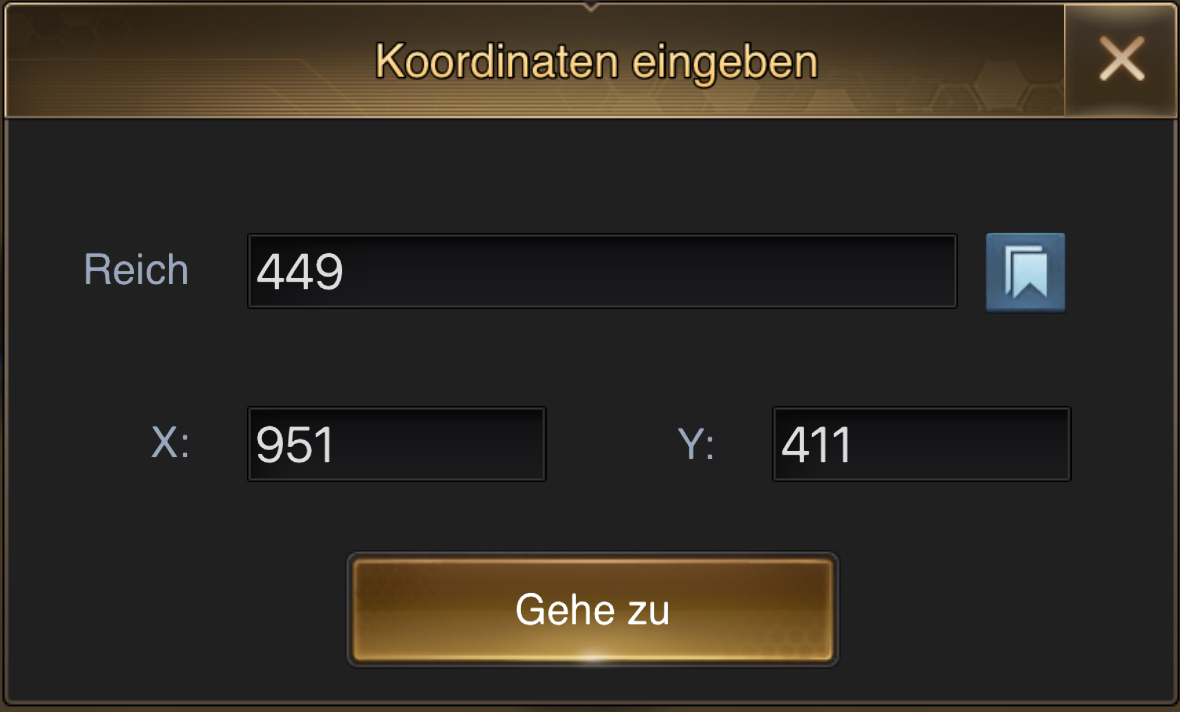
\includegraphics[width=5cm]{Bilder/IMG_E0004.JPG}
  \caption{Koordinaten Eingabe}
  \label{fig:koordinaten}
\end{figure}

Wenn du dann im Staat \#449 bist, klickst du in einem freien Bereich, um die Optionen zu sehen. Normalerweise kommt Rechts ein
Button „Staat wechseln“, den wählst du an und bestätigst.  (Abbildung~\ref{fig:zone})

\begin{figure}[H] 
  \centering
     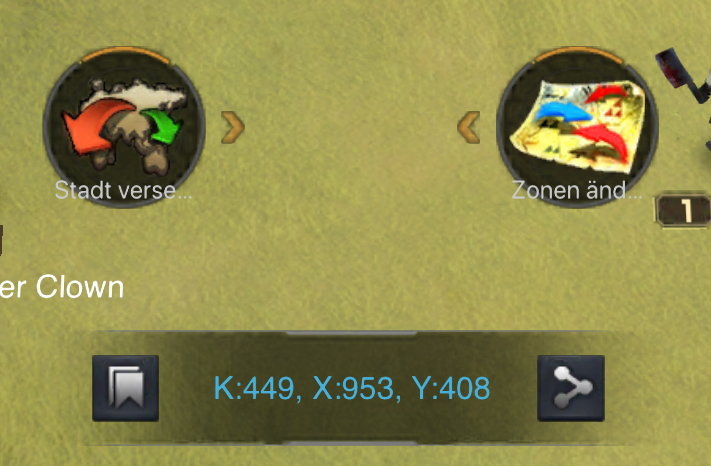
\includegraphics[width=3cm]{Bilder/IMG_E0005.JPG}
  \caption{Zone ändern}
  \label{fig:zone}
\end{figure}

Jetzt sollte deine Basis irgendwo in unserem Staat sein. Damit kannst du dich jetzt für unsere Farm Allianz bewerben.
Du hast auch nur 14 Tage Zeit um den Staat zu wechseln.
Du kannst nach unser Allianz suchen oder auf eine Basis der Allianz klicken [(PaT) daWahnsinn (X:951, Y:411)] oder mich per PM anschreiben,
damit wir dich einladen können.
Wichtig! Der Allianz Teleport funktioniert nur einmal! Danach kostet er 2000 Diamanten! Also am besten gar nicht erst in eine
andere Allianz eintreten.

\subsection{Basis Layout}

Wenn man mehrere Farmen hat, ist es sinnvoll das Layout der Basis gleich zu haben. SO findet man sich bei Bedarf schnell zurecht.
Es ist darauf zu achten, einzelne Bereiche so anzulegen, das man sie leicht von der Straße trennen kann. In Abbildung~\ref{fig:map}
sind zum Beispiel die Lager mit nur einer Straße zur Basis verbunden. Diese kann man bei Bedarf schnell auftrennen um ungewollte Plünderung
zu verhindern. Auch alle nicht genutzten Gebäude sind so verbunden, damit man sie schnell anbinden kann falls man etwas daran machen muß.

\begin{figure}[H] 
  \centering
     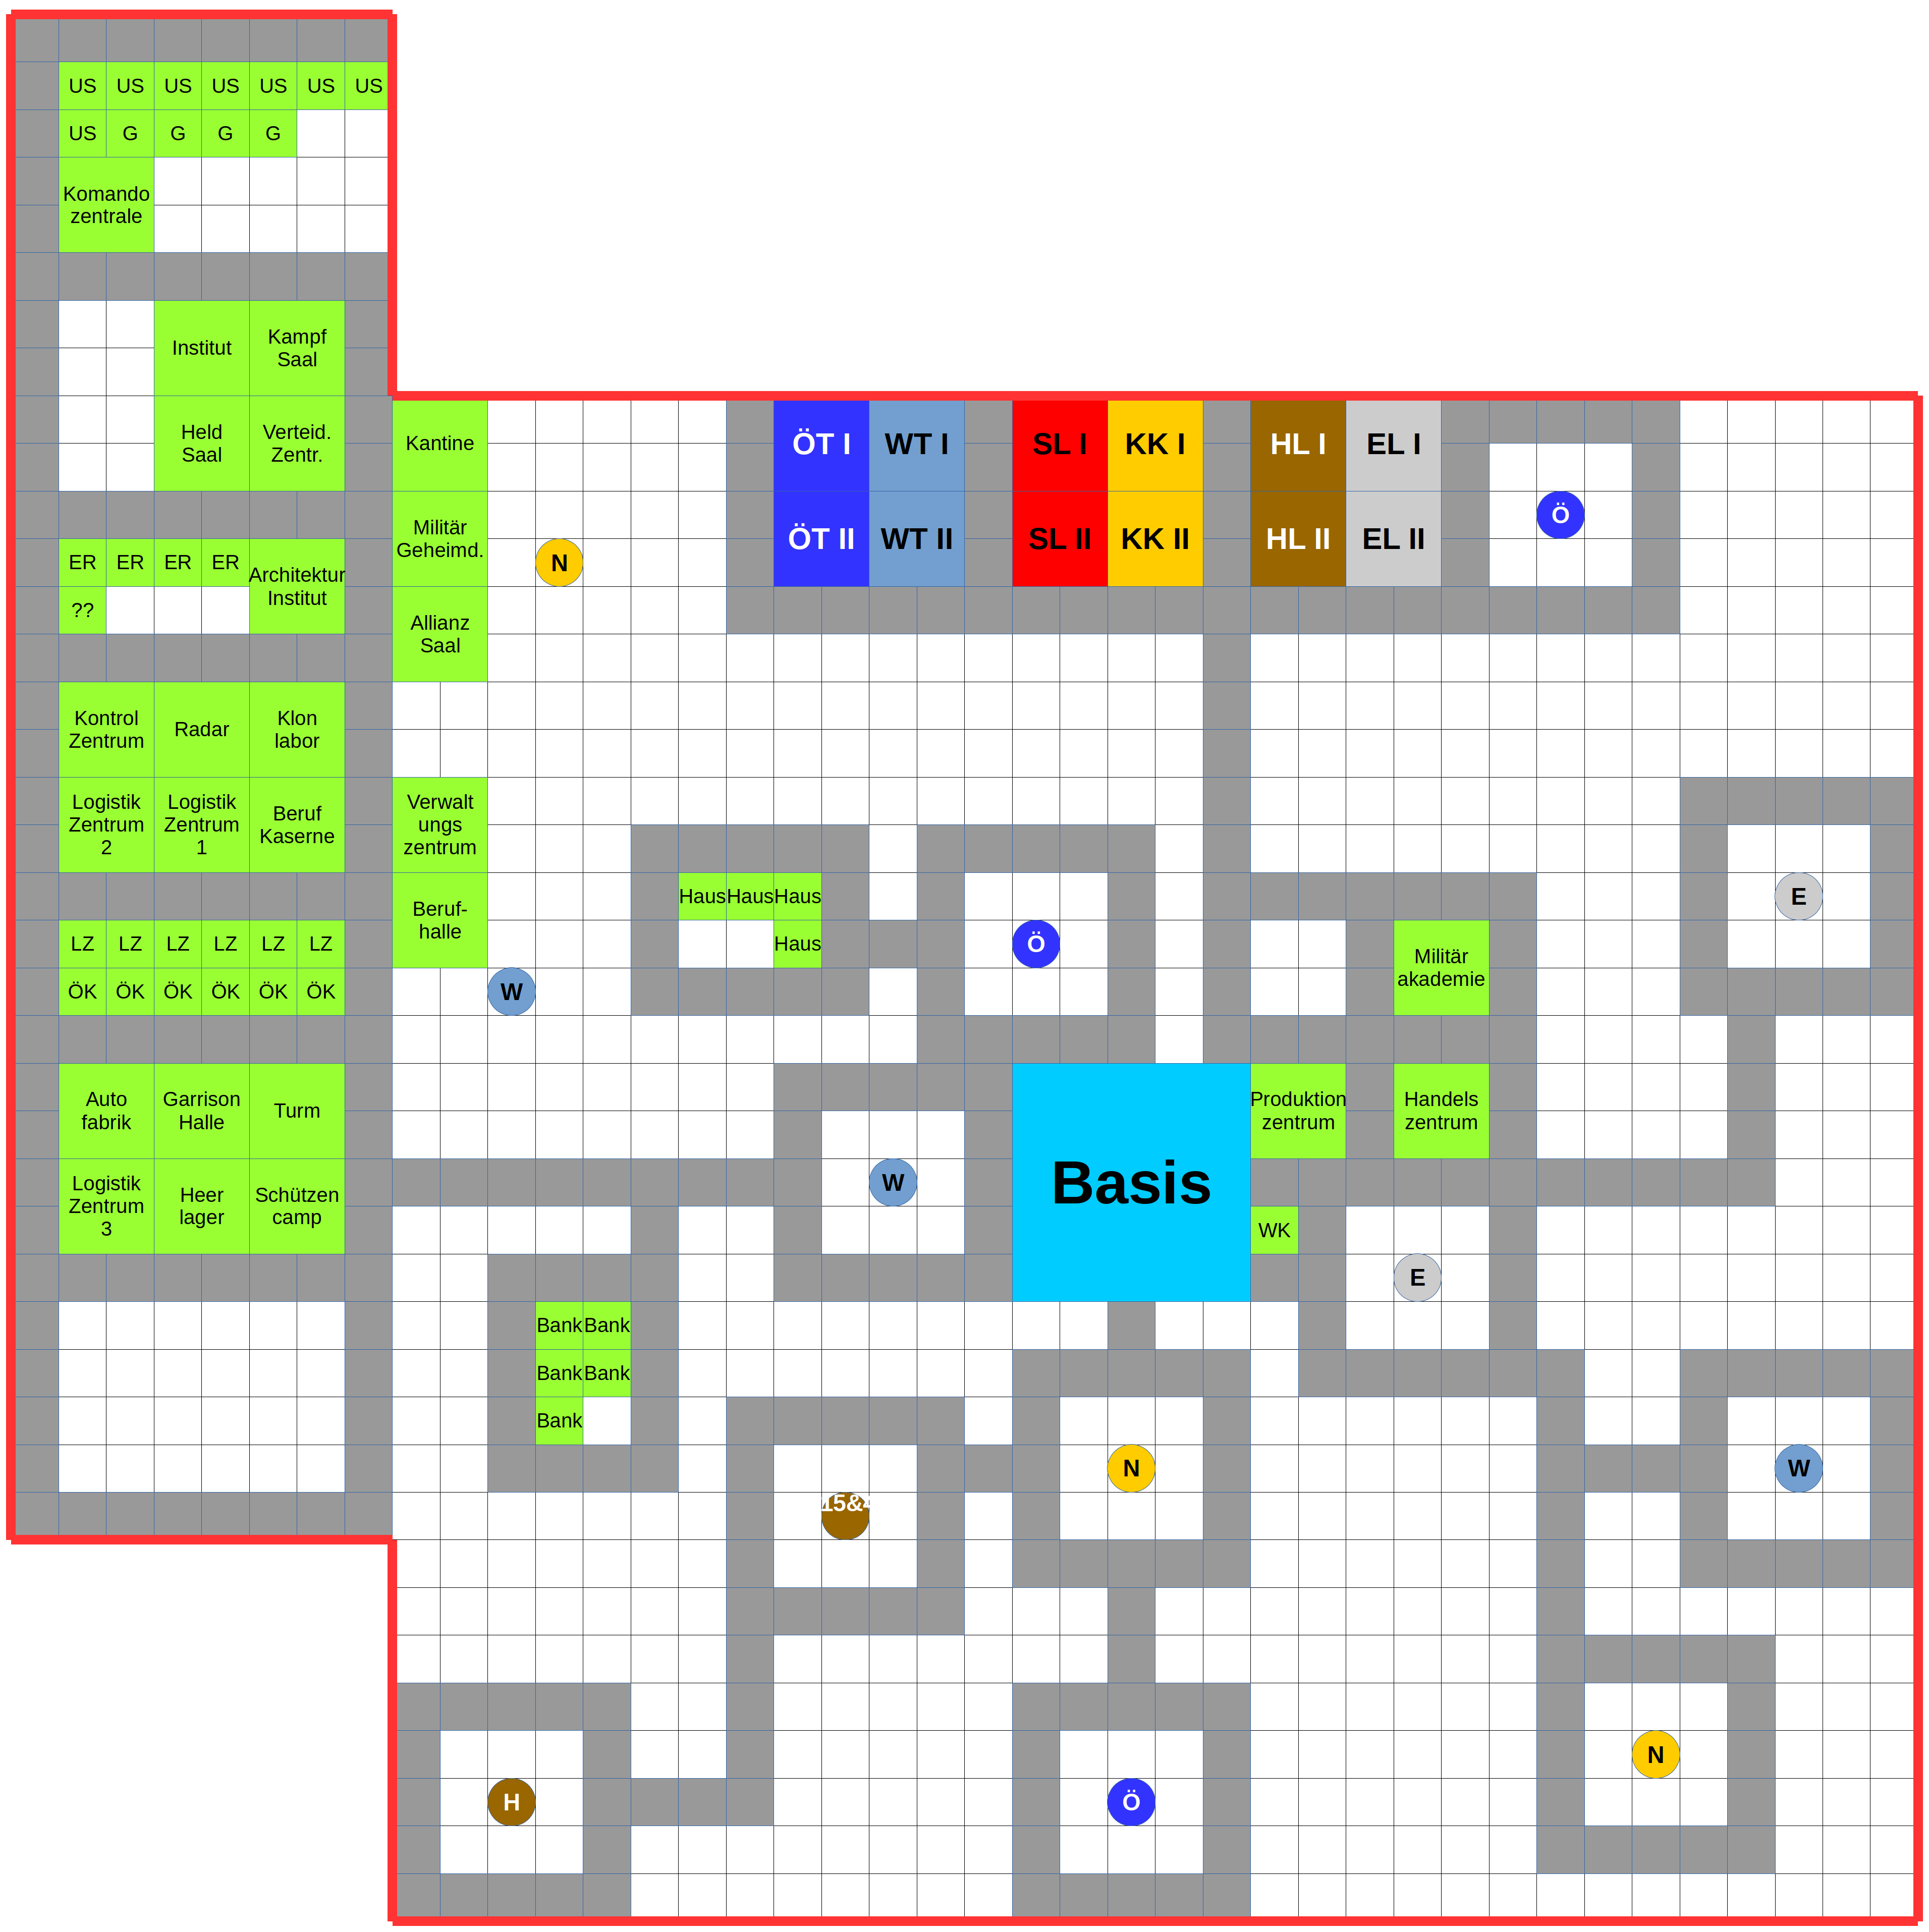
\includegraphics[width=0.8\textwidth]{Bilder/map.png}
  \caption{Basis Layout}
  \label{fig:map}
\end{figure}

\subsection{Benutzer}
Spätestens beim Eintritt in eine Allianz wirst du nach deinem Benutzernamen gefragt.
Diesen kann man einmalig unter Einstellungen -> Benutzerprofil ändern. Danach kostet es 2.000 Diamanten.
Also gut überlegen welchen Namen man wählt und aufpassen, das man sich nicht vertippt.

Es wird empfohlen, den Namen seines Main-Accounts zu wählen und Farm mit einer Nummer anzuhängen. Siehe Abbildung~\ref{fig:benutzer}.

\begin{figure}[H]
  \centering
     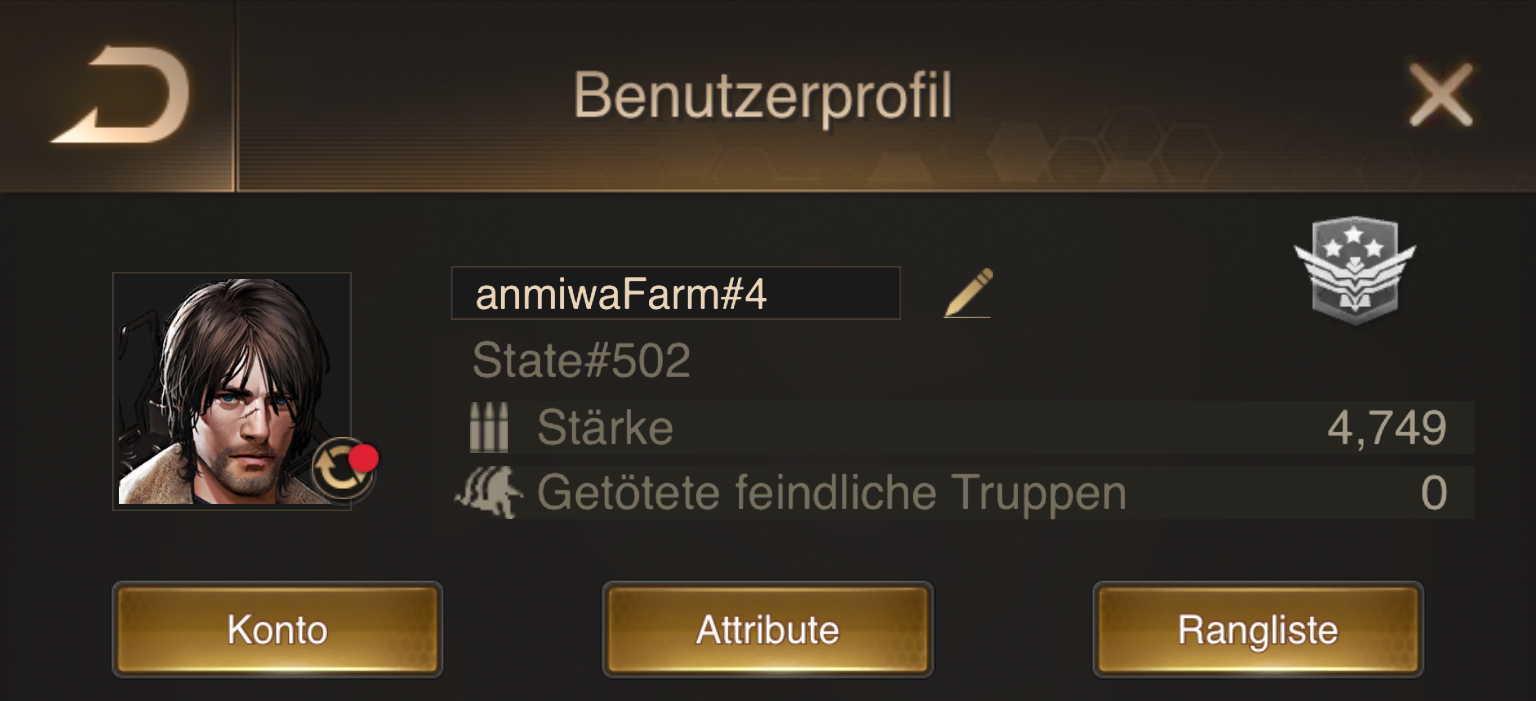
\includegraphics[width=5cm]{Bilder/IMG_E0006.JPG}
  \caption{Benutzerprofil ändern}
  \label{fig:benutzer}
\end{figure}

\subsection{Flagge}
Als Flagge empfehle ich die der UN. Es wäre schön, wenn sich allgemein die Regel etablieren würde, das Basen mit der UN Flagge nicht angegriffen werden dürfen.
Ändern kann man die Flagge unter Einstellungen -> Fahne. Das kostet nichts und kann beliebig oft gemacht werden.

\subsection{Mehrere (Farm-) Konten erstellen}
Man kann in LastShelter mehrere Konten mit derselben E-Mail anlegen. Dazu müssen nur Punkte in der E-Mail an beliebiger Stelle vor dem @ eingefügt werden.
Ist deine E-Mail z. B. max.mustermann@gmail.com dann sind gültige Kombinationen: 

\begin{itemize}
  \item m.ax.mustermann@gmail.com
  \item max.m.ustermann@gmail.com
  \item max.muster.mann@gmail.com
\end{itemize}	

Du bekommst immer eine Mail auf deine richtige Addresse, welche du dann bestätigen musst.
So lassen sich beliebig viele Konten mit derselben Adresse erstellen. Das Passwort sollte der Einfachheit halber immer dasselbe sein, muss aber nicht. (Aufschreiben!)


\section{Wartung}

Wenn man viele Farmen besitzt macht es keinen Sinn mehr, diese täglich zu besuchen.
Bei 30 Farmen kann man schnell 1 - 2 Stunden mit Wartung verbringen. Solange man nur 3 - 5 Farmen hat kann man das noch machen, wenn man will.

\subsection{Wartungsfreie Farm}
Wenn man eine Farm Wartungsfrei betreiben will, gibt es ein paar Dinge zu beachten.

\begin{itemize}
  \item Halte den Stromverbrauch niedrig. Entferne die Straße von allen Gebäuden die nicht notwendig sind.
  \item Wenn die Farm fertig ist (alles notwendige auf max), bringe die Bevölkerungszahl auf maximum und entferne anschließend die Straße von der Kantine.
  \item Starte mit Bauer um die Farm schneller aufzubauen. Wähle dann, wenn du fertig bist, als Beruf Händler.
        Dieser bekommt 50\% mehr Geld. Das gleicht die auf Grund fehlender Nahrung auf 66\% gefallene Geldproduktion aus.
\end{itemize}	

%Da du ja nicht täglich das Produktion Ztr. leeren willst, 

\subsection{Gewartete Farm}
Für eine täglich gewartete Farm, macht es Sinn, sich Morgends und Abends einmal einzuloggen. Der Abstand sollte größer als 12 Stunden betragen.

Morgends:
\begin{itemize}
  \item Ernte im Produktion Ztr.
  \item Schnell Produktion aller Ressourcen Produktions Icons
  \item Wasser Überschuß im Handelszentrum verkaufen
  \item Freie Helden abholen
\end{itemize}	
Abends:
\begin{itemize}
  \item Ernte im Produktion Ztr.
  \item Schnell Produktion aller Ressourcen Produktions Icons
  \item Hubschrauber rufen und Wasser Überschuß im Handelszentrum verkaufen.
  \item Freie Helden abholen
\end{itemize}	


\subsection{Schnell Produktion}
Die Schnell Produktion steht einmal am Tag mit 100\% zur Verfügung. Mit genügend Zeit dazwischen, kann man diese ein zweites mal mit hoher Erfogsaussicht starten.
Für jede Ressourcen sind dabei ca. 50k Ernte möglich.


\subsection{Produktion Ztr.}
Alle 12 Stunden kann man eine Ernte über das Produktion Zentrum starten. Bei Vollausbau auf Level 15 ist diese durchaus ergiebig (Abbildung~\ref{fig:ernte}).
Um diese optimal zu nutzen, muß man sich natürlich etwa alle 12 Stunden in die Farm einloggen.
\begin{figure}[H] 
  \centering
     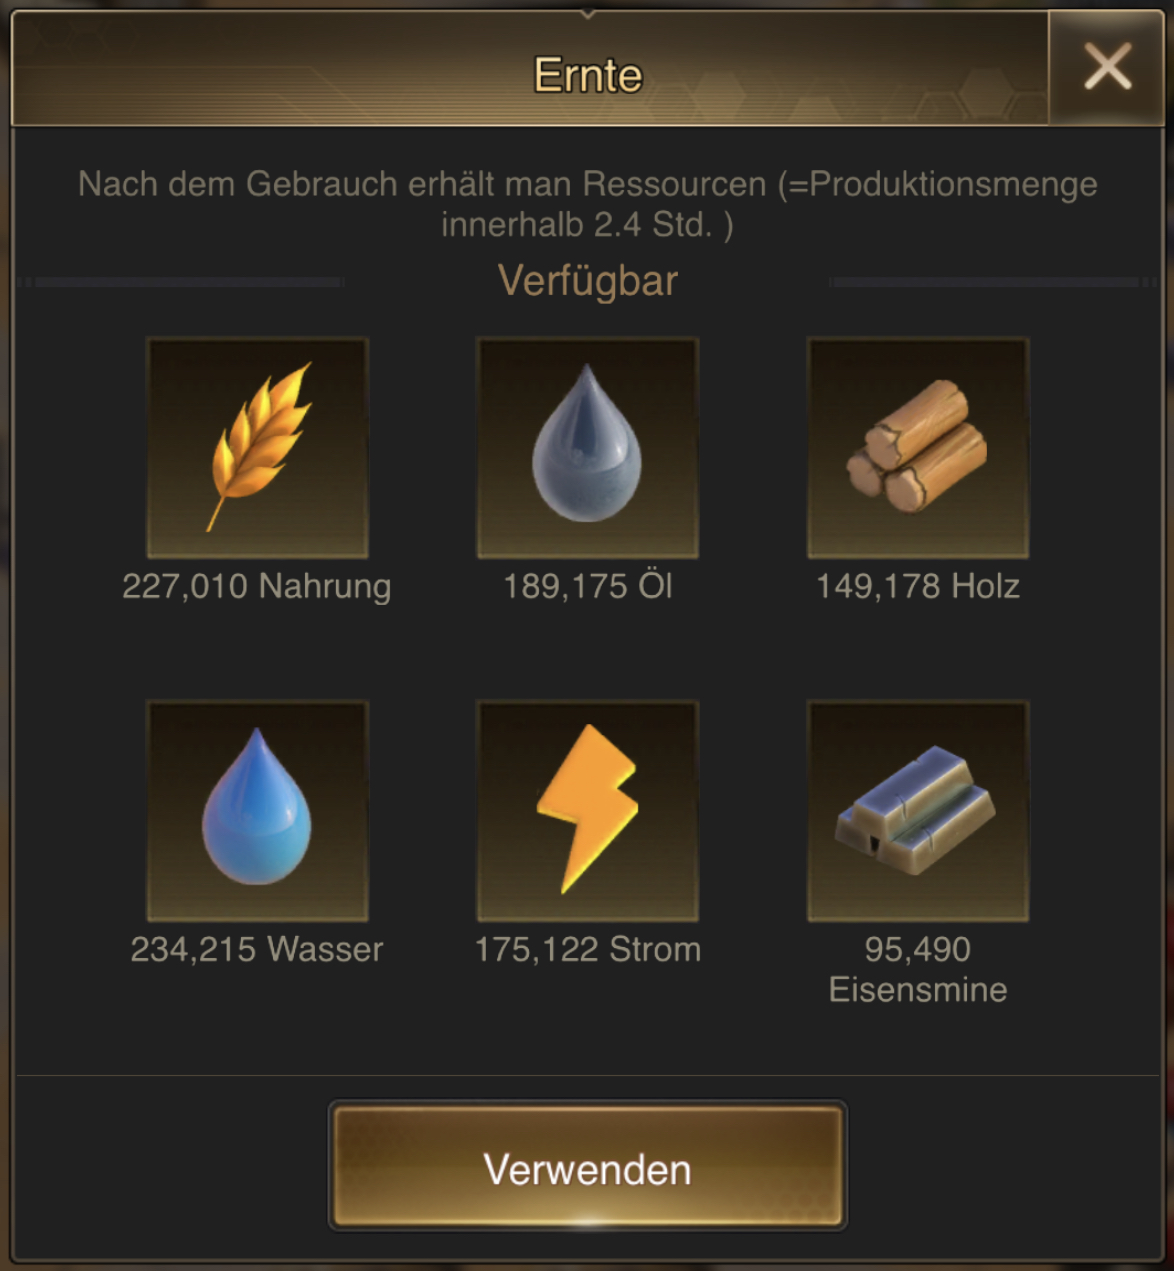
\includegraphics[width=6cm]{Bilder/IMG_E0014.JPG}
  \caption{Ernte im Produktion Ztr.}
  \label{fig:ernte}
\end{figure}


\subsection{Helden-Event}
\label{Heldenevent}
Der Event "`Helden ausbilden"' ist jeden Donnerstag und Sonntag im Eventzentrum unter "`Spieler-Wettrüstung"' verfügbar. (Abbildung~\ref{fig:helden})

\begin{figure}[H] 
  \centering
     \includegraphics[width=6cm]{Bilder/IMG_0031.PNG}
  \caption{Event: Helden ausbilden}
  \label{fig:helden}
\end{figure}

Um die 2.600.000 Punkte für die dritte Kiste zu bekommen, könnte man folgendermaßen vorgehen:

\begin{table}[h!]
  \centering
    \begin{tabularx}{0.7\textwidth}{lcrr}
      Aufgabe & Anzahl & Punkte & Summe \\
      \hline
      Normale Rekrutierungskarte & 10 & 10.000 & 100.000 \\
      Elite Rekrutierungskarte & 2 & 50.000 & 100.000 \\
      Super Rekrutierungskarte & 1 & 200.000 & 200.000 \\
      Medaillen austauschen & 600 & 1.000 & 600.000 \\
      Fähigkeit freischalten & 10 & 20.000 & 200.000 \\
      Medaille verbrauchen & 700 & 2.000 & 1.400.000 \\
      \hline
      ~ & ~ & ~ & 2.600.000 \\
    \end{tabularx}
  \caption[Event]{Beispiel Event}
\end{table}

Wie du siehst, ist es also machbar, und in wenigen Minuten erledigt.
Folgende Vorgehensweise empfehle ich dir dabei:

\begin{itemize}
  \item Hole dir jeden Tag deine drei freien Helden ab, aber tausche nicht die Heldenkarten ein.
  \item Zerlege und Tausche regelmäßig Helden um. lass aber genügend für Donnerstag über, damit du in der Militärakademie maximal Medaillen tauschen kannst.
  \item Nutze EXP um den Helden auf Level 6 zu bringen, dann kannst du ein Fähigkeit freischalten.
  \item Upgrade den Helden mit Wisdom Medaillen bis du keine mehr hast. Benutze alle Fähigkeiten eines Helden um möglichst wenig Medaillen übrig zu lassen.
  \item Zerlege den Helden jetzt. Dadurch bekommst du einen Teil der Medaillen zurück.
  \item Wiederhole die letzten drei Schritte bist du die dritte Kiste hast oder alle Medaillen verbraucht sind.
  \item Falls dir die Helden ausgehen: Zerlege alle Helden die du hast, lasse keine Stationiert oder im APC. 
        Wenn du jetzt das Spiel beendest und neu startest, hast du wieder einen blauen. Wiederhole das bis du genügend Helden hast.
  \item Stelle sicher dass das Event gestartet ist bevor du anfängst.
  \item Während des CSB-Event kannst du die Events für bestimmte Tage auswählen. Nimm "`Helden ausbilden"' dann kannst du am Donnerstag doppelt abkassieren.
\end{itemize}	

Der Aufwand lohnt sich, sieh dir die Belohnungen (Abbildung~\ref{fig:belohnung}) in der dritten Kiste an.

\begin{figure}[H] 
  \centering
     \includegraphics[width=6cm]{Bilder/IMG_0032.PNG}
  \caption{Belohnung 3. Kiste}
  \label{fig:belohnung}
\end{figure}



\subsubsection{Empfohlene Gebäude Level}

Nachfolgend eine Liste der benötigten Gebäude und der jeweiligen Level.

\begin{table}[h!]
  \centering
\begin{tabularx}{1.0\textwidth}{lcccX}
  Gebäude & Anzahl & Level & Straße & Bemerkung \\
  \hline
  Basis & 1 & 15 & ja & Nicht höher als 15, da sonst die Punkte für die dritte Kiste bei den Events stak ansteigen. \\
  Windkraftwerk & 1 & 15 & ja & Genügt knapp um die Basis mit Strom zu versorgen. \\
  Handelszentrum & 1 & 15 & ja & Hier wird Wasser und Strom verkauft. \\
  Militärakademie & 1 & 15 & ja & Um die gesammelten Helden in Medaillen umzutauschen für die Events. \\
  Produktion Ztr. & 1 & 15 & ja & Wenn man Bauer ist, kann hier täglich viele Ressourcen bekommen. 
                                  Allerdings müsste man sich dazu täglich einloggen.\\
  Farm & 6 & 15 & ja & Nahrung zum plündern. \\
  Sägewerk & 6 & 15 & ja & Holz zum plündern. \\
  Klärwerk & 5 & 15 & ja & Wasser zum verkaufen. \\
  Ölquelle & 5 & 15 & ja & Öl zum plündern. \\
  Eisenmine & 5 & 15 & ja & Eisen zum plündern. \\
  Wohnhaus & 5 & 15 & ja & Bevölkerung für die Bank-Effizienz.
                           Um alle Gebäude frei zu schalten, muss die Bevölkerungszahl über 55k gebracht werden. \\
  Bank & 5 & 15 & ja & Geld zum plündern. \\
  Garage & 4 & ~ & nein & Baufahrzeuge. \\
  Lager & 1 & 15 & ja & Alle Lager I auf Level 10, damit man Lager II bekommt. \\
  Lager II & 1 & 3 & ja & Die Kosten für höhere Level lohnen sich meist nicht. 
                          Wenn man regelmäßig seine Farm plündert, sollten 6M Lagerkapazität genügen. \\
\end{tabularx}
\caption[Gebäude]{Die Gebäude einer Farm}
\end{table}

\begin{table}[h!]
  \centering
\begin{tabularx}{1.0\textwidth}{lcccX}
  Gebäude & Anzahl & Level & Straße & Bemerkung \\
  \hline
  Institut     & 1 & 8 & nein & Wird benötigt um Stadtentwicklung auf MAX zu bringen. \\
  Öl-Kraftwerk & 5 & 9 & nein & Eins wird auf Level 9 benötigt um den Stromspeicher auf Level 10 upgraden zu können. 
                                Die anderen 4 können auf Level 1 bleiben.\\
  Schützencamp & 1 & 13 & nein & Wird benötigt um Basis auf Level 14 upgraden zu können. \\
  Unterschlupf & 1 & 8 & nein & Einer wird auf Level 8 benötigt um Basis auf Level 9 upgraden zu können.
                                Die anderen können auf Level 1 bleiben.\\
  Lazarett     & 1 & 9 & nein & Eines wird auf Level 9 benötigt um Basis auf Level 10 upgraden zu können.
                            Die anderen können auf Level 1 bleiben.\\
  Kantine      & 1 & 14 & nein & Wird benötigt um Basis auf Level 15 upgraden zu können. \\
  Held Saal    & 1 & 15 & nein & Wird benötigt um Militärakademie auf Level 15 upgraden zu können. \\
  Verteidigungszentrum & 1 & x & nein & Hier sollte man ein Level wählen, um mit dem APC des Main 3 mal plündern zu können. \\
  Restliche Gebäude & ~ & 1 & nein & Werden nicht benötigt und verbraucht sonst Ressourcen. \\
\end{tabularx}
\caption[Gebäude]{Die Gebäude einer Farm}
\end{table}



\subsection{Items}

\begin{description}
  \item[Nahrung:] Wird gefarmt und steht zum Plündern bereit.
  \item[Wasser:] Dient nur zum Verkauf über das Handelszentrum (Hubschrauber)
  \item[Öl:] Wird gefarmt und steht zum plündern bereit.
  \item[Strom:] Wird dringend benötigt, um alles am Laufen zu halten. Die geringe Unterproduktion des Windrades muss durch wöchentliches auffüllen eines Ölkraftwerkes ausgeglichen werden.
  \item[Holz:] Wird gefarmt und steht zum Plündern bereit.
  \item[Eisen:] Wird gefarmt und steht zum Plündern bereit.
  \item[Geld:] Wird gefarmt und steht zum Plündern bereit.
  \item[Bevölkerung:] Wird für Geld Produktion benötigt. Ohne tägliches Auffüllen der Kantine sinkt die Bevölkerung auf 66\%, was für Händler ausreichen ist.
  \item[Diamanten:] Werden in großen Mengen durch Heldentausch Trick gewonnen
  \item[Truppen:] Diese werden nicht benötigt und würden nur Nahrung verschwenden
\end{description}



\section{Tips \& Tricks}

\begin{itemize}
  \item Farmen nur bis maximal Level 15 hochrüsten, da sonst die täglichen Events für die dritte Kiste zu teuer wird.
  \item Händler bekommen zwar weniger Ressourcen, aber 50\% mehr Geld. Wenn man sich nicht täglich um die Farm kümmern möchte, lieber Händler nehmen. Sonst natürlich Bauer.
  \item Windkraftwerk immer auf höchstem Level, um möglichst lange ohne Interaktion (Öl auffüllen) auszukommen.
  \item Alles was man nicht braucht von der Straße entfernen. Spart Strom.
  \item Wenn man die maximale Bevölkerungszahl erreicht hat, kann man die Kantine leer werden lassen und die Straße entfernen. Die Bevölkerung sinkt dann auf 66\% wie auch die Geldproduktion. Durch die 50\% plus des Händlers, hat man wieder 100\%.
  \item Die Lager II bis maximal Level 3, da diese dann extrem teuer werden. 7M sollten genügen.
\end{itemize}	


\end{document}






